\documentclass[10pt, conference, letterpaper]{IEEEtran}

\usepackage{algorithm}
\usepackage{algorithmicx}
\usepackage{algpseudocode}
\usepackage{amsfonts}
\usepackage{amsmath}
\usepackage{amssymb}
\usepackage[ansinew]{inputenc} 
\usepackage{xcolor}
\usepackage{mathtools}
\usepackage{graphicx}
\usepackage{caption}
\usepackage{subcaption}
\usepackage{import}
\usepackage{multirow}
\usepackage[export]{adjustbox}
\usepackage{breqn}
\usepackage{mathrsfs}
\usepackage{acronym}
%\usepackage[keeplastbox]{flushend}
\usepackage{setspace}
\usepackage{bm}
\usepackage{stackengine}
\usepackage{tikz}
\usepackage[margin=1in]{geometry}
\usepackage{seqsplit}
\usepackage{booktabs}
\usepackage[table]{xcolor}
\usepackage{url}
\usepackage[backend=biber,style=numeric,citestyle=numeric]{biblatex}
\addbibresource{biblio.bib}
\usepackage{hyperref}
\usepackage{float}
\usepackage{siunitx}
\usepackage{xspace}
\usepackage{tabularx}
\usepackage{microtype}
\usepackage{array}
\usepackage{pdflscape}
\usepackage{longtable}
\usepackage{subfiles}

\hypersetup{
    colorlinks=true,
    linkcolor=blue,
    citecolor=blue,
    filecolor=magenta,
    urlcolor=cyan,
    breaklinks=true,
    pdfauthor={Your Name},
    pdftitle={Your Title},
}


\usepackage{listings}

\lstset{%
 backgroundcolor=\color[gray]{.85},
 basicstyle=\small\ttfamily,
 breaklines = true,
 keywordstyle=\color{red!75},
 columns=fullflexible,
}%

\lstdefinelanguage{BibTeX}
  {keywords={%
      @article,@book,@collectedbook,@conference,@electronic,@ieeetranbstctl,%
      @inbook,@incollectedbook,@incollection,@injournal,@inproceedings,%
      @manual,@mastersthesis,@misc,@patent,@periodical,@phdthesis,@preamble,%
      @proceedings,@standard,@string,@techreport,@unpublished%
      },
   comment=[l][\itshape]{@comment},
   sensitive=false,
  }

\usepackage{listings}

% listings settings from classicthesis package by
% Andr\'{e} Miede
\lstset{language=[LaTeX]Tex,%C++,
    keywordstyle=\color{RoyalBlue},%\bfseries,
    basicstyle=\small\ttfamily,
    %identifierstyle=\color{NavyBlue},
    commentstyle=\color{Green}\ttfamily,
    stringstyle=\rmfamily,
    numbers=none,%left,%
    numberstyle=\scriptsize,%\tiny
    stepnumber=5,
    numbersep=8pt,
    showstringspaces=false,
    breaklines=true,
    frameround=ftff,
    frame=single
    %frame=L
}

\renewcommand{\thetable}{\arabic{table}}
\renewcommand{\thesubtable}{\alph{subtable}}

\DeclareMathOperator*{\argmin}{arg\,min}
\DeclareMathOperator*{\argmax}{arg\,max}

\def\delequal{\mathrel{\ensurestackMath{\stackon[1pt]{=}{\scriptscriptstyle\Delta}}}}

\graphicspath{{./figures/}}
\setlength{\belowcaptionskip}{0mm}
\setlength{\textfloatsep}{8pt}

\newcommand{\eq}[1]{Eq.~\eqref{#1}}
\newcommand{\fig}[1]{Fig.~\ref{#1}}
\newcommand{\tab}[1]{Tab.~\ref{#1}}
\newcommand{\secref}[1]{Section~\ref{#1}}

\newcommand\MR[1]{\textcolor{blue}{#1}}
\newcommand\red[1]{\textcolor{red}{#1}}
\newcommand{\mytexttilde}{{\raise.17ex\hbox{$\scriptstyle\mathtt{\sim}$}}}

%\renewcommand{\baselinestretch}{0.98}
% \renewcommand{\bottomfraction}{0.8}
% \setlength{\abovecaptionskip}{0pt}
\setlength{\columnsep}{0.2in}

% \IEEEoverridecommandlockouts\IEEEpubid{\makebox[\columnwidth]{PUT COPYRIGHT NOTICE HERE \hfill} \hspace{\columnsep}\makebox[\columnwidth]{ }} 

\title{Functional and Structural Characterization of a protein domain family }

\author{
    \begin{tabular}{cc}
        \textbf{Alberto Calabrese} & \textbf{Marlon Helbing} \\
        \small Data Science, Department of Mathematics, University of Padova & \small Data Science, Department of Mathematics, University of Padova \\
        \small Email: \texttt{alberto.calabrese.2@studenti.unipd.it} & \small Email: \texttt{marlonjoshua.helbing@studenti.unipd.it} \\[1.5em]
        \multicolumn{2}{c}{\textbf{Lorenzo Baietti}} \\
        \multicolumn{2}{c}{\small Data Science, Department of Mathematics, University of Padova} \\
        \multicolumn{2}{c}{\small Email: \texttt{lorenzo.baietti@studenti.unipd.it}}
    \end{tabular}
}

\IEEEoverridecommandlockouts

\newcounter{remark}[section]
\newenvironment{remark}[1][]{\refstepcounter{remark}\par\medskip
   \textbf{Remark~\thesection.\theremark. #1} \rmfamily}{\medskip}

\begin{document}

\maketitle

\begin{abstract}
This study focuses on the characterization of the protein domain family associated with Pfam identifier \texttt{PF00151}, specifically the Lipase/vitellogenin domain in \textit{Homo sapiens}. We constructed a Position-Specific Scoring Matrix (PSSM) and a Hidden Markov Model (HMM) to represent the domain, evaluated them against SwissProt annotations, and analyzed their functional and structural aspects. The models effectively captured conserved sequence features, and predictions matched well with known annotations. The results emphasize the domain's critical biological roles and suggest avenues for further refinement and exploration.
\end{abstract}

% !TEX root = template.tex

\section{Introduction}
\label{sec:introduction}

The domain of a protein is an important part to model, as it can evolve, function and exist independently of the rest of the protein chain~\cite{domain_structure}. Therefore, in this work, we aim to characterize the domain of a \textit{Homo sapiens} protein that is linked to Lipase/Vitellogenin by building a sequence model starting from a single sequence and providing a functional characterization of the entire domain family. This report is structured as follows. In Section II, we describe how we built both a PSSM~\cite{psiblast} and an HMM~\cite{hmmer} model, which are then evaluated in their performance on the protein and residue level against SwissProt~\cite{uniprot} proteins annotated with the 'ground truth' Pfam domain~\cite{pfam} in Section III. Next, we looked at functional and structural properties of the entire protein family, such as taxonomy in Section IV, function in Section V, and finally motifs in Section VI.  In Section VII we report results and a conclusion is provided in Section VII.


% !TEX root = template.tex

\section{Model Building}

Given our initial data (Table~\ref{tab:protein_info}) and the representative domain sequence (Fig.~\ref{fig:sequence}), we collected $1000$ homologous sequences by means of a BLAST search~\cite{blast} against the UniProt Knowledgebase (UniProtKB)~\cite{uniprot} with an e-value threshold of $0.0001$. Next, we utilized ClustalOmega~\cite{clustalomega} to generate a multiple sequence alignment. To have a more generalizable and performant model later on, we cleaned the MSA by first removing redundant rows at a $100$\%\ threshold using JalView~\cite{jalview}, resulting in $155$ sequences, and then performing a detailed conservation analysis. In particular, for the HMM model input, we first removed columns of residues(? maybe called different) that had $90$\%\ or more gaps, which resulted in roughly removing $70$\%\ of the initially $3254$ columns. For the PSSM model input, ... (lorenzo). Given the filtered MSAs, we then proceeded to build both the HMM~\cite{hmmer} and PSSM models using HMMER-3.4~\cite{hmmer} and NCBI-BLAST+~\cite{ncbi-blast}, respectively.

\begin{table}[h]
    \centering
    \caption{Protein Domain Information}
    \label{tab:protein_info}
    \begin{tabular}{ll}
        \toprule
        \textbf{Property} & \textbf{Value} \\
        \midrule
        UniProt ID & P54315 \\
        PfamID & PF00151 \\
        Domain Position & 18-353 \\
        Organism & Homo sapiens (Human) \\
        Pfam Name & Lipase/vitellogenin \\
        \bottomrule
    \end{tabular}
\end{table}

\begin{figure}[h]
    \centering
    \caption{Domain Sequence}
    \label{fig:sequence}
    \footnotesize
    \seqsplit{KEVCYEDLGCFSDTEPWGGTAIRPLKILPWSPEKIGTRFLLYTNENPNNFQILLLSDPSTIEASNFQMDRKTRFIIHGFIDKGDESWVTDMCKKLFEVEEVNCICVDWKKGSQATYTQAANNVRVVGAQVAQMLDILLTEYSYPPSKVHLIGHSLGAHVAGEAGSKTPGLSRITGLDPVEASFESTPEEVRLDPSDADFVDVIHTDAAPLIPFLGFGTNQQMGHLDFFPNGGESMPGCKKNALSQIVDLDGIWAGTRDFVACNHLRSYKYYLESILNPDGFAAYPCTSYKSFESDKCFPCPDQGCPQMGHYADKFAGRTSEEQQKFFLNTGEASNF}
\end{figure}

% !TEX root = template.tex

\section{Model Evaluation}

To generate predictions, we used HMM-SEARCH and PSI-BLAST with default parameters. Both searches were performed against the manually curated SwissProt database (release $29.11.2024$)~\cite{uniprot}, resulting in $83$ predicted proteins with e-values $< 0.05$ and their corresponding domain locations within each protein sequence. Since HMM-SEARCH returned multiple domain hits, we only selected the one with the smallest e-value. To generate the ground truth, we collected all 82 reviewed proteins in SwissProt annotated with the given Pfam domain~\cite{pfam} utilizing the InterPro API~\cite{interpro}. We evaluated both models against the ground truth using two approaches. First, at the protein level, we verified whether predicted proteins matched the annotated ones. Second, at the residue level, for proteins present in both our predictions and the SwissProt reviewed set, we created binary vectors representing domain positions and compared them to quantify the overlap of domain boundary predictions. To assess the performance of the model, we calculated precision, recall, F-score, balanced accuracy and MCC. Results are reported in section VII.







% !TEX root = template.tex

\section{Taxonomy}

To understand the taxonomic distribution of proteins within our family, we utilized a systematic approach to collect and analyze lineage data for the $83$ sequences found in our family. Using the protein identifiers obtained from PSI-BLAST~\cite{psiblast} and HMM-SEARCH~\cite{hmmer}, we queried the UniProt API~\cite{uniprot_api} to fetch the complete taxonomic lineage for each protein. This process captured the hierarchical classification of each protein within its biological domain, from the broadest category (e.g., \textit{Eukaryota}) to the most specific organism classification, and allowed for representation using the Newick tree format~\cite{newick_format} (Fig.~\ref{fig:phylo-tree}). Several interesting patterns can be observed in the graph.

The collected lineage data was then processed to calculate frequency counts for each taxonomic level. By traversing the hierarchical taxonomy, we were able to generate a nested dictionary representing the occurrence of each taxonomic node across the dataset. This allowed for a detailed visualization of taxonomic diversity.

The taxonomic tree was plotted using the ETE Toolkit~\cite{ete_toolkit}, leveraging the Newick format derived from the hierarchical data. Node sizes in the phylogenetic tree were adjusted to reflect the relative abundance of each taxonomic entity, with larger nodes indicating higher representation in the protein family. (Fig.~\ref{fig:phylo-tree}) Illustrates the resulting phylogenetic tree, showcasing the distribution of proteins across various taxonomic groups. Notable clusters include a strong representation within mammals, particularly in the order \textit{Primates}, as well as significant diversity within arthropods.


\begin{figure*}[h!]
    \centering
    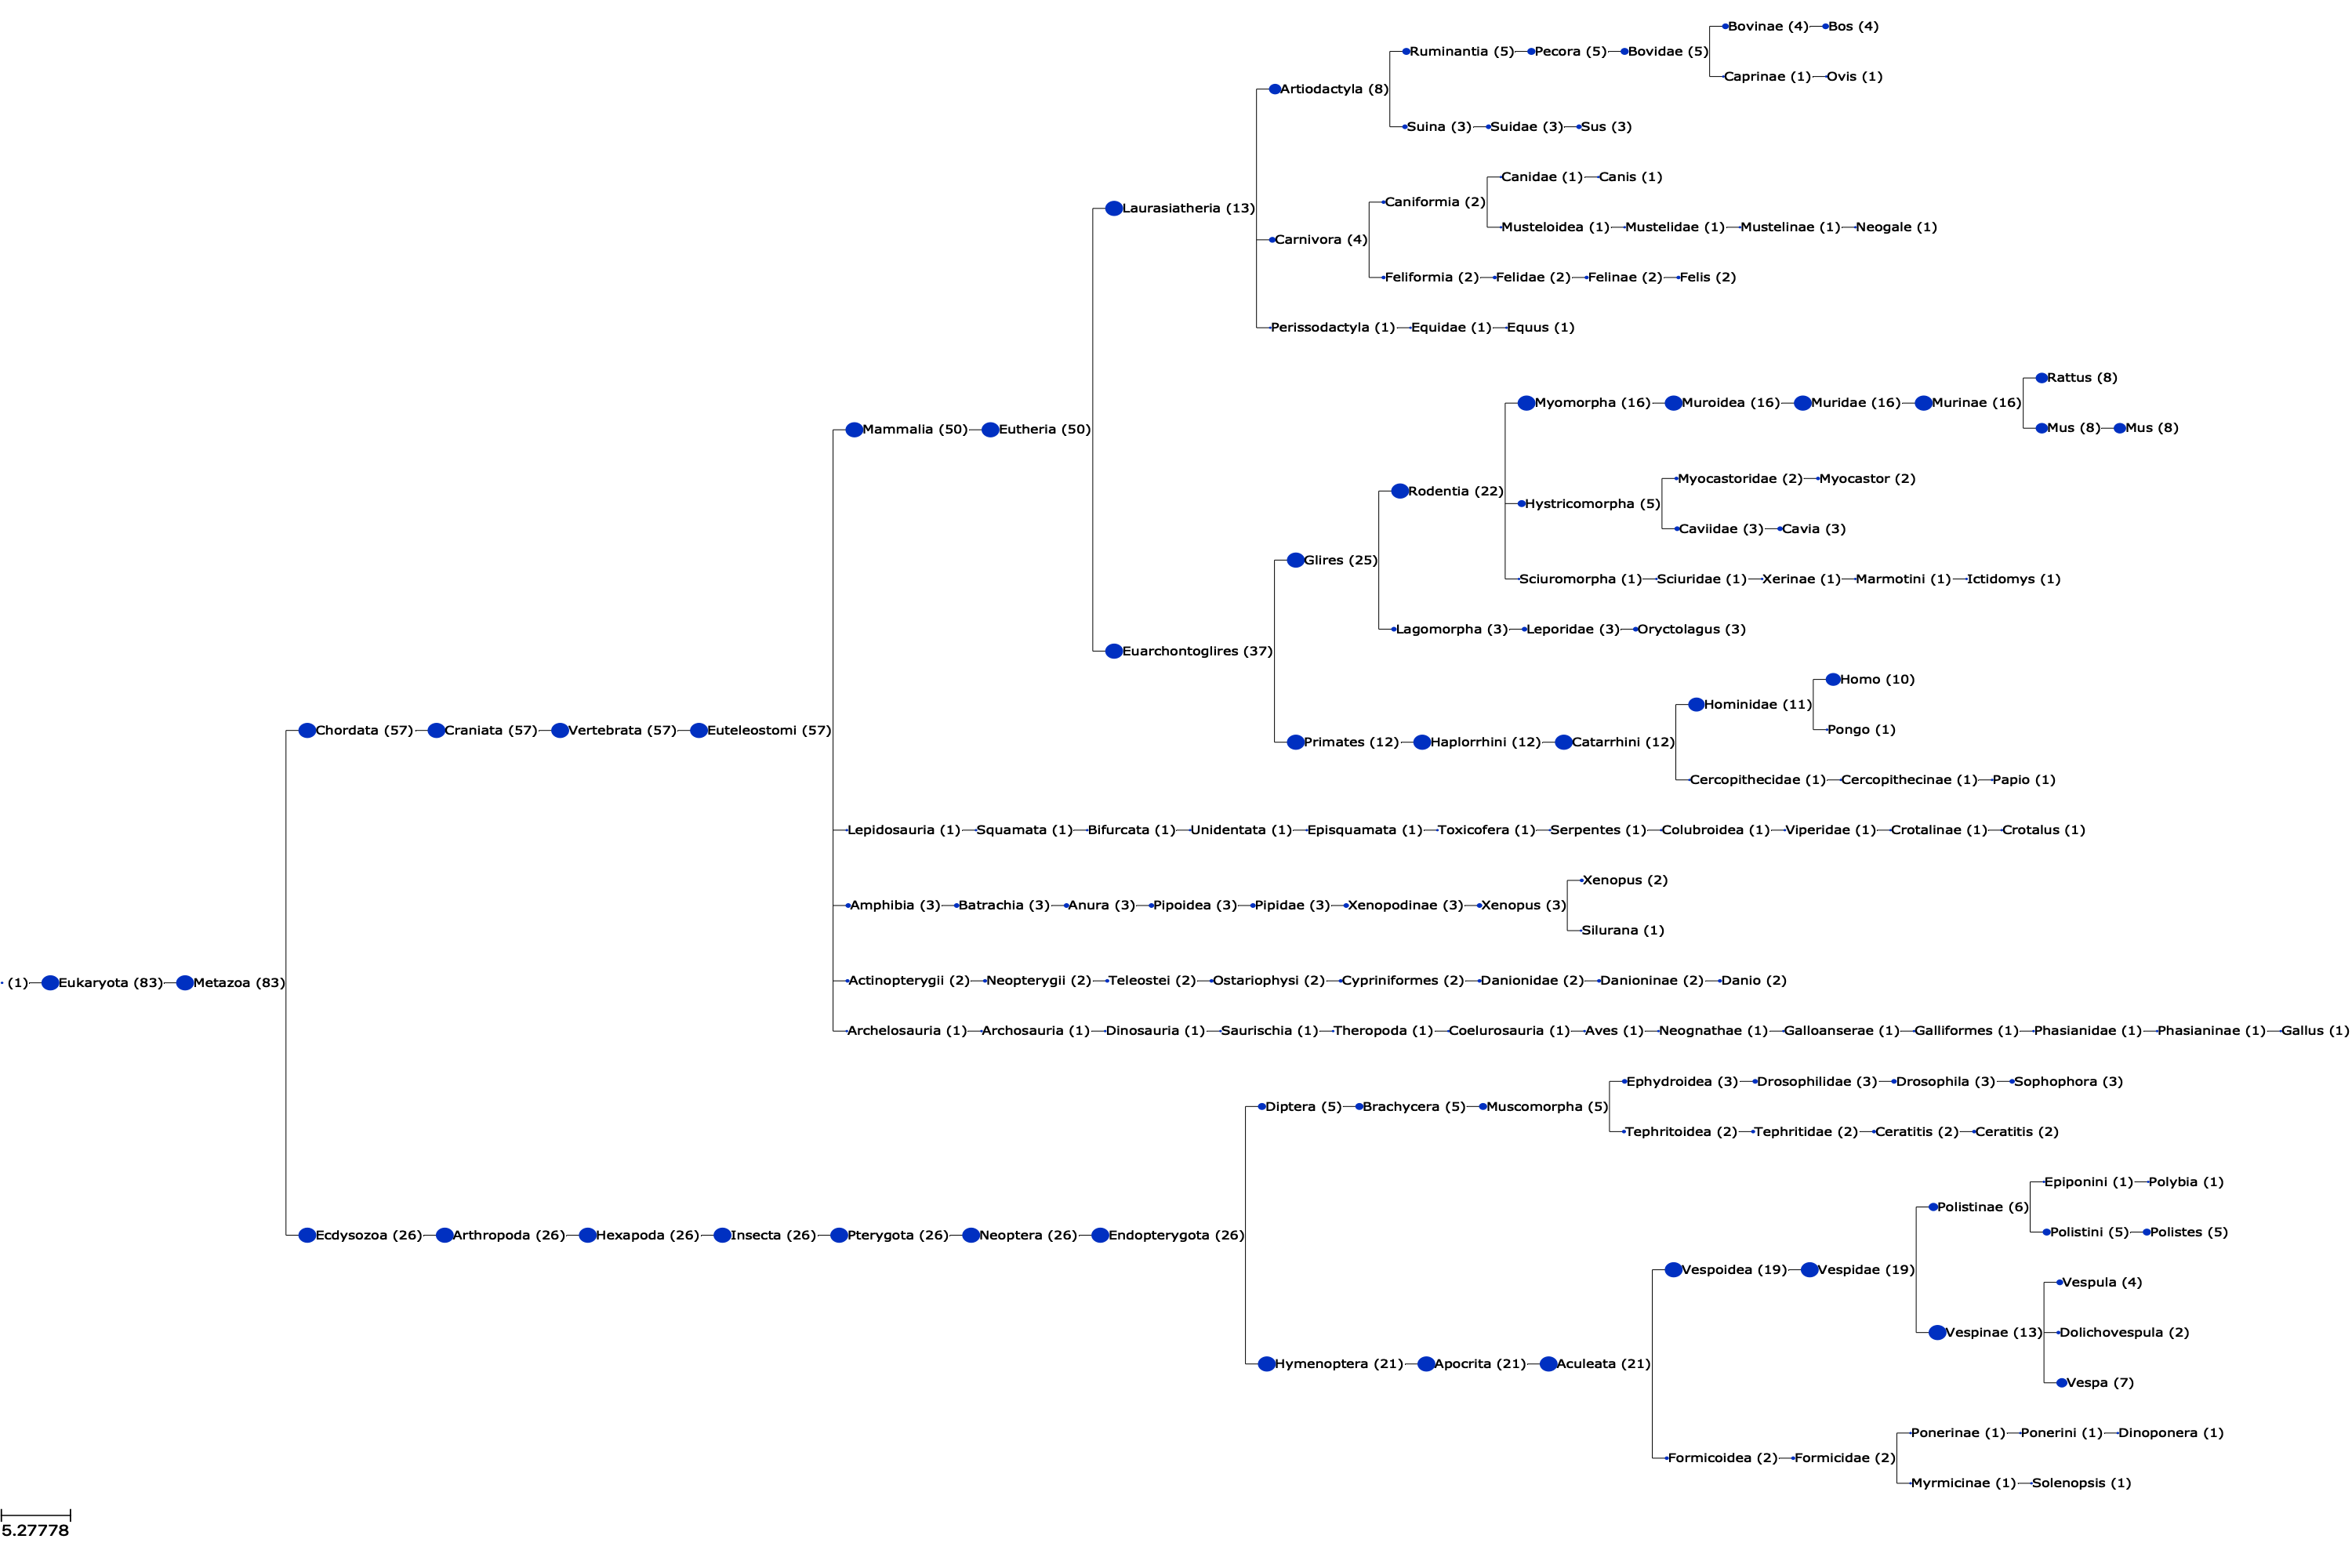
\includegraphics[width=0.8\textwidth]{images/phylogenetic_tree_freq.png}
    \caption{Phylogenetic tree illustrating taxonomic relationships across family sequences, with node sizes reflecting relative abundance. The tree highlights a dominant presence in mammals, particularly \textit{Primates}, and significant diversity within arthropods. This visualization underscores the evolutionary adaptation and taxonomic distribution of the protein domain.}
    \label{fig:phylo-tree}
\end{figure*}

% !TEX root = template.tex
\section{Function}

First, we obtain GO annotations~\cite{gene_ontology} for both our family proteins and the entire SwissProt database. To have a more complete representation, we then expanded these GO annotations by parsing the ontology tree~\cite{obo_parser} and adding the ancestor GO terms of each initially found GO term. In order to calculate the enrichment of each GO term in our family compared to the ones found in the SwissProt database, we used Fisher's exact test~\cite{fisher_test}. We used a $2 \times 2$ contingency table where rows indicated the presence or absence of a GO term and columns differentiated between proteins within and outside our domain family (Table~\ref{tab:contingency}). 
\begin{table}[h!]
    \centering
    \small
    \begin{tabular}{lccc}
        \toprule
         & Protein in family & \multicolumn{2}{c}{Protein not in family} \\
        \\
        \midrule
        Has GO term & $a$ & \multicolumn{2}{c}{$b$} \\
        No GO term & $c$ & \multicolumn{2}{c}{$d$} \\
        \bottomrule
    \end{tabular}
    \caption{Contingency table}
    \label{tab:contingency}
\end{table}
For each GO term, we tested two hypotheses. Under the null hypothesis, the proportion of proteins annotated with that given GO term in our domain family equals the proportion in the full SwissProt dataset. We evaluated this against two alternative hypotheses: a right-tailed test to detect enrichment (higher proportion in our family than in SwissProt) and a two-tailed test to detect any significant difference in proportions (either higher or lower). The enrichment value was then calculated as:
$$
\dfrac{family\_proportion}{swissprot\_proportion}
$$
We generated a word cloud visualization using the enriched terms (where $p < 0.05$ for both $p_{\text{two-tailed}}$ and $p_{\text{right-tailed}}$ tests) weighted by their enrichment value (Fig.~\ref{fig:go-wordcloud}). Furthermore, we reported the most enriched branches of the ontology tree based on the enriched terms. For each GO term, we parsed the ontology tree~\cite{obo_parser} up to the root and added the GO term itself as an enriched child to each found ancestor. After this process, we selected only branches - which we defined as the immediate parent of a GO term, or the GO term itself in case of a root term - that had more than $2$ enriched children and a maximum depth of $3$ to filter for high-level terms. A selection of $10$ of these branches, ranked by their cumulative significance score $S = \sum -\log_{10}(p_{\text{two-tailed}})$ calculated across all child terms, can be seen in Table~\ref{tab:go_terms}.


\begin{figure*}[h!]
    \centering
    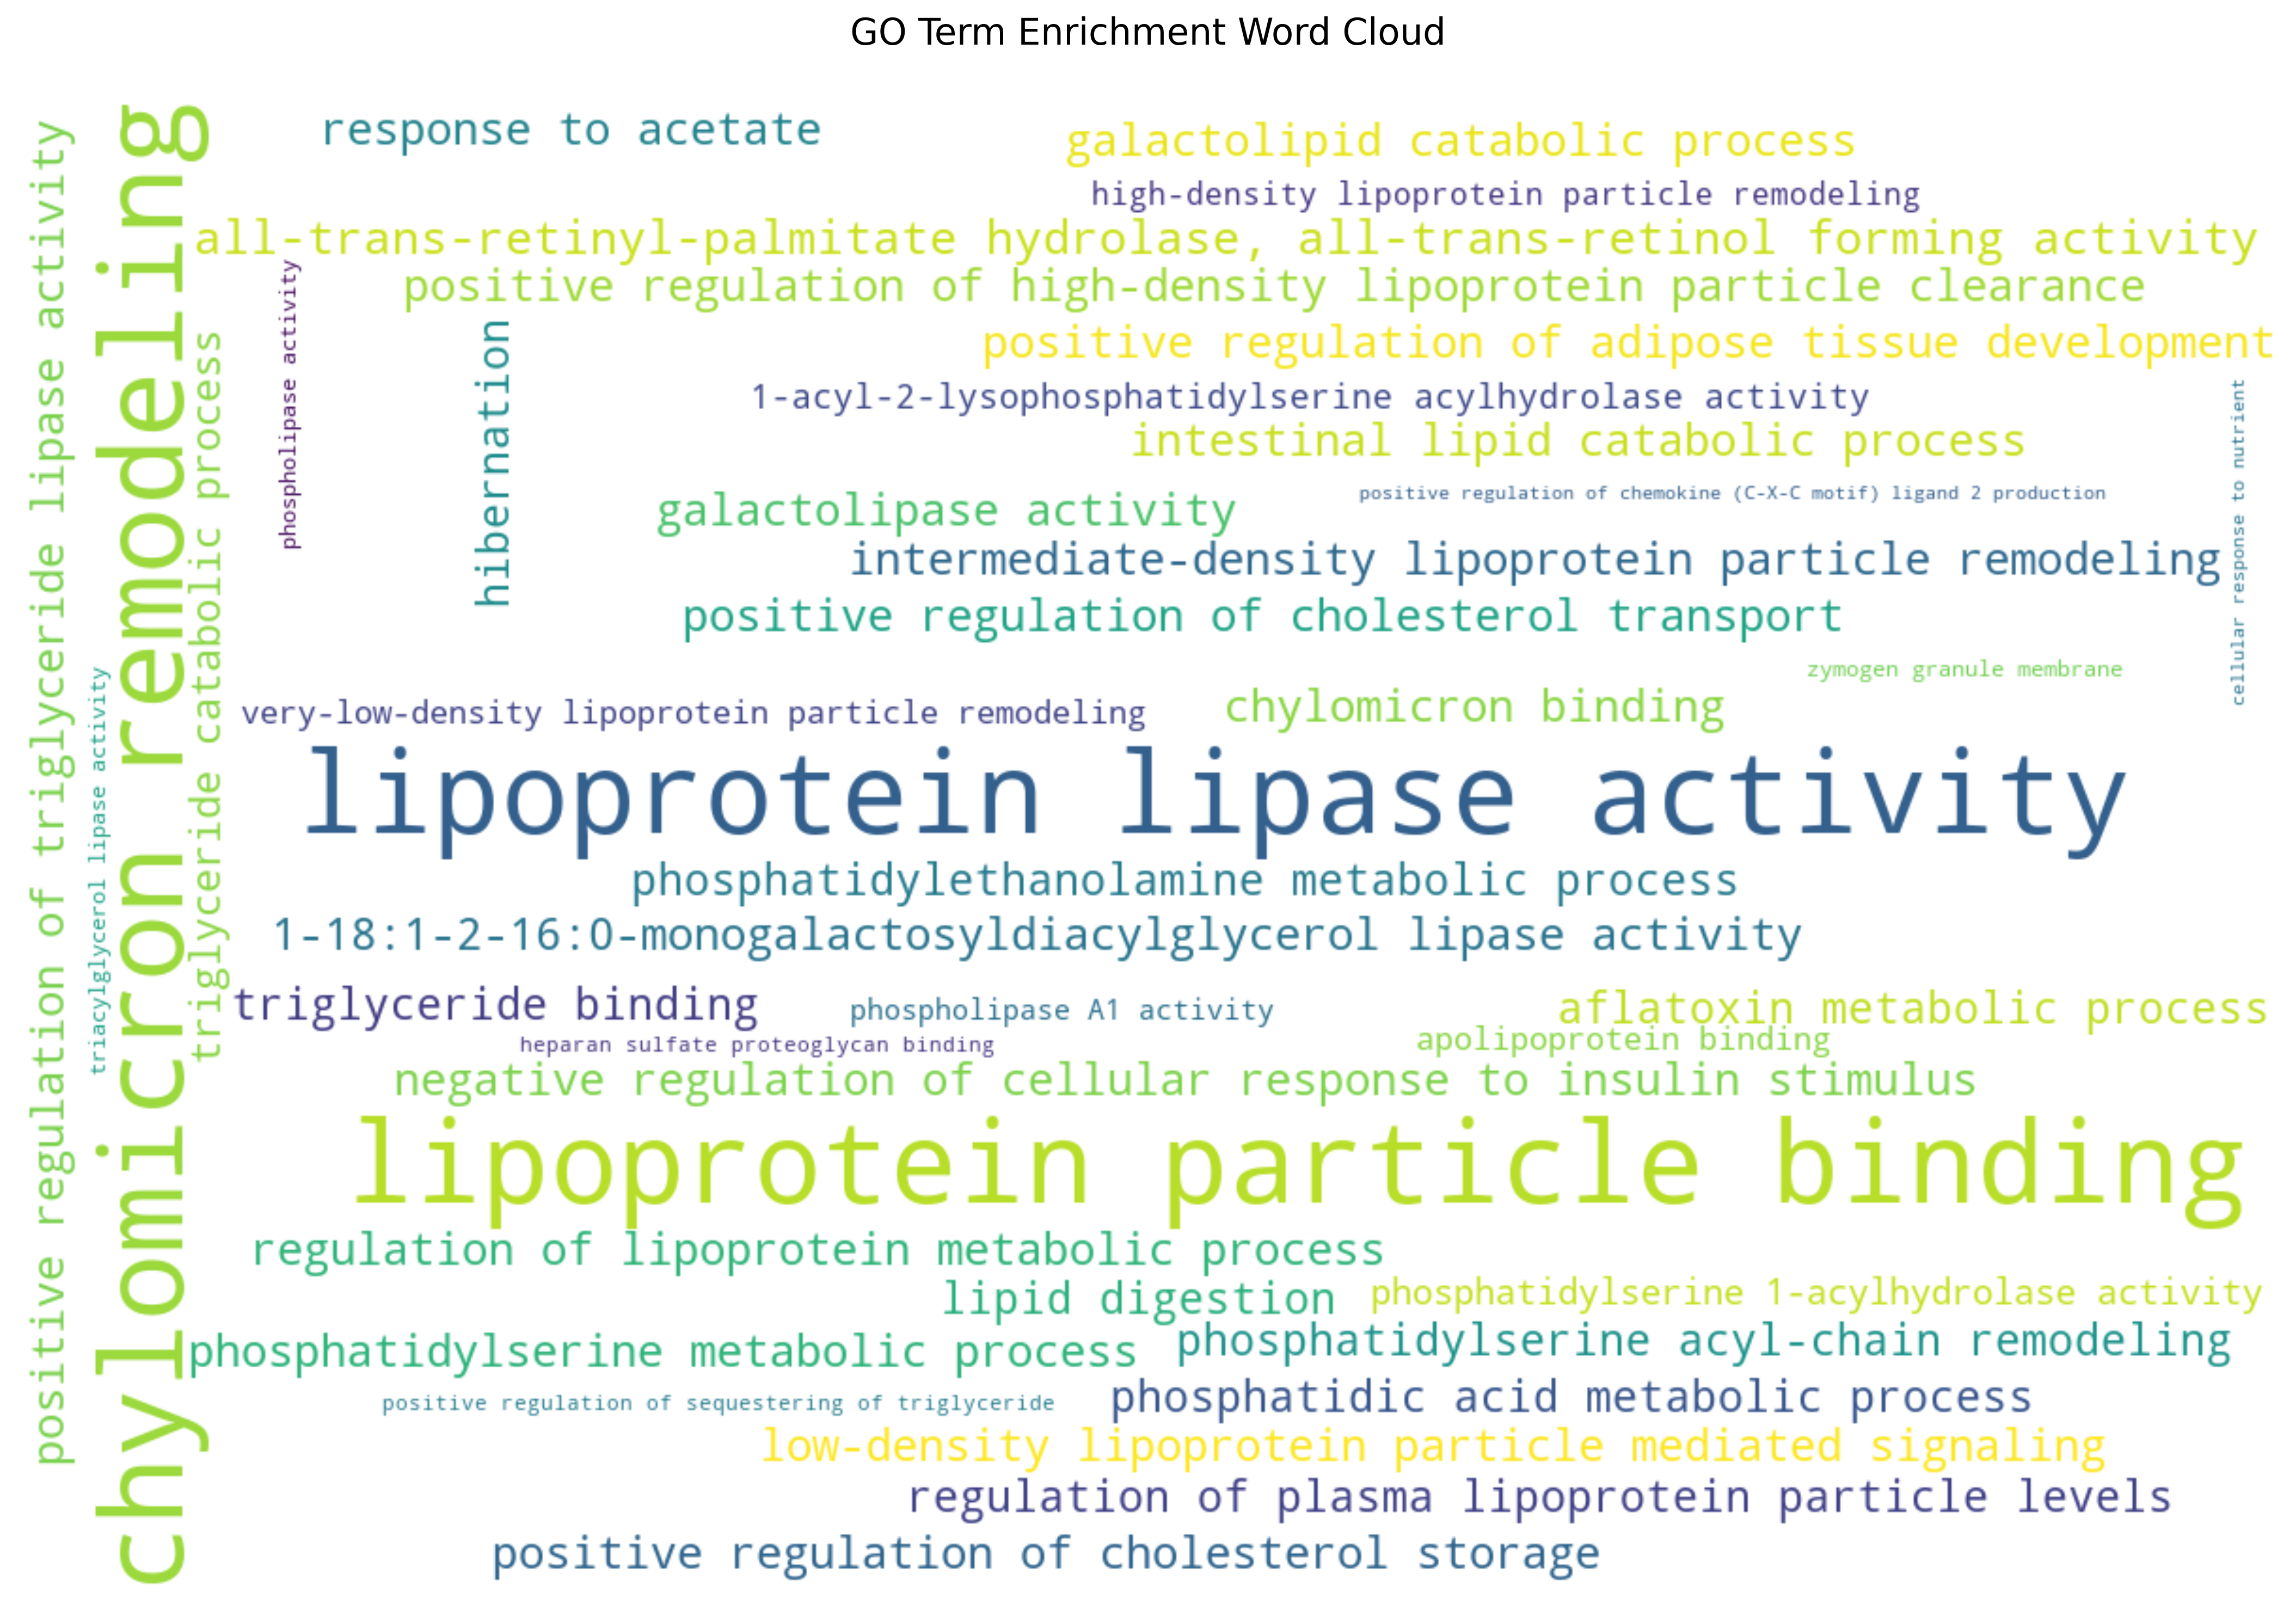
\includegraphics[width=0.8 \textwidth]{images/go_enrichment_wordcloud.png}
    \caption{Word cloud visualization of enriched GO terms. The size of each term represents its relative frequency or significance, with larger text indicating higher enrichment. Terms are related to lipoprotein metabolism, lipase activity, and various cellular processes.}
    \label{fig:go-wordcloud}
\end{figure*}

% !TEX root = template.tex
\section{Motifs}

To identify conserved short motifs within our protein family, we began by analyzing the locations of intrinsically disordered regions. These regions were predicted using MobiDB-lite~\cite{mobidb}, which combines multiple approaches to consensus disorder prediction. The analysis focused on regions likely to contain functional motifs. We then extracted motif patterns from two widely-used resources: ELM classes~\cite{elm} and ProSite patterns~\cite{prosite}. For ProSite patterns, a script adapted from Stevin Wilson's \texttt{PrositePatternsToPythonRegex}~\cite{stevin_wilson} project was used to convert motif patterns into Python-compatible regular expressions. This enabled efficient motif matching within the disordered regions. Overall, our workflow ensured comprehensive coverage of short linear motifs (SLiMs) known to play roles in protein-protein interactions and regulatory mechanisms. The identified motifs were cataloged for further analysis.



%\newpage
\section{Results}

\subsection{Model Evaluation}
We evaluated the performance of PSI-BLAST and HMM-SEARCH models at both the protein and residue levels against the SwissProt database. At the protein level, both models successfully identified $82$ ground truth proteins, with only one false positive and no false negatives (Table~\ref{tab:confusion}). This indicates high precision and recall for both methods. At the residue level, the PSSM model demonstrated higher precision and F-scores compared to the HMM model, although the HMM model achieved similar recall values, particularly in detecting conserved residues (Table~\ref{tab:metrics}).

\begin{table}[H]
    \centering
    \small
    \caption{Confusion Matrices for PSI-BLAST and HMM at Protein and Residue Levels}
    \label{tab:confusion}
    \begin{tabular}{llrrrr}
        \toprule
        \textbf{Level} & \textbf{Method} & \textbf{TP} & \textbf{FP} & \textbf{FN} & \textbf{TN} \\
        \midrule
        \multirow{2}{*}{Protein} 
        & PSI-BLAST & 82 & 1 & 0 & 0 \\
        & HMM & 82 & 1 & 0 & 0 \\
        \midrule
        \multirow{2}{*}{Residue} 
        & PSI-BLAST & 23,393 & 2,247 & 1,622 & 2,352 \\
        & HMM & 23,287 & 5,578 & 1,728 & 2,280 \\
        \bottomrule
    \end{tabular}
\end{table}

\begin{table}[H]
    \centering
    \small
    \caption{Performance Metrics for PSI-BLAST and HMM at Protein and Residue Levels}
    \label{tab:metrics}
    \begin{tabular}{lcccc}
        \toprule
        \multirow{2}{*}{\textbf{Metric}} & \multicolumn{2}{c}{\textbf{Protein Level}} & \multicolumn{2}{c}{\textbf{Residue Level}} \\
        \cmidrule(lr){2-3} \cmidrule(lr){4-5}
        & PSI-BLAST & HMM & PSI-BLAST & HMM \\
        \midrule
        Precision & 0.9880 & 0.9880 & 0.9124 & 0.8068 \\
        Recall & 1.0000 & 1.0000 & 0.9352 & 0.9309 \\
        F-score & 0.9939 & 0.9939 & 0.9236 & 0.8644 \\
        Bal. Acc. & 0.5000 & 0.5000 & 0.7233 & 0.6105 \\
        MCC & 0.0000 & 0.0000 & 0.4745 & 0.2882 \\
        \bottomrule
    \end{tabular}
\end{table}

The superior performance of the PSSM model can be attributed to its ability to capture position-specific amino acid conservation patterns effectively. However, the HMM model's underperformance may reflect the challenges posed by a relatively small training dataset of $155$ sequences and the need for further optimization of its parameters.

\subsection{Taxonomy Analysis}
We visualized the taxonomic distribution of the protein family using data from UniProt~\cite{uniprot}, plotted as a phylogenetic tree (Fig.~\ref{fig:phylo-tree}). The tree revealed a strong focus within \textit{Chordata} ($n=57$), particularly in \textit{Mammalia} ($n=50$). The main clusters within mammals include \textit{Rodentia} ($n=22$) and \textit{Primates} ($n=12$). These results suggest that the domain is well-conserved across mammalian lineages, which may reflect its fundamental roles in lipid metabolism and energy regulation. The clustering of \textit{Rodentia} and \textit{Primates} further highlights the domain's relevance in key biological functions across diverse species. 

\subsection{Gene Ontology Enrichment}
Our GO enrichment analysis revealed several significant terms related to lipid metabolism and cellular processes. The most enriched function was \textit{intermediate-density lipoprotein particle remodeling} (Fig.~\ref{fig:go-wordcloud}), followed by terms such as \textit{chylomicron remodeling} and \textit{intestinal lipid catabolic process}. These terms point to the domain's involvement in lipid processing and dietary fat metabolism. Additional enriched terms included \textit{lipoprotein lipase activity}, which emphasizes the domain's functional role in lipid regulation and enzymatic activity. These findings align with previous research on the biological significance of the domain in lipid-related pathways. The hierarchical structure of enriched GO branches (Table~\ref{tab:go_terms}) further highlights its specialization in metabolic and catalytic processes.

\begin{table}[H]
    \centering
    \resizebox{1\linewidth}{!}{%
    \begin{tabular}{|l|l|c|c|c|}
        \hline
        \textbf{GO Term} & \textbf{Branch Name} & \textbf{Depth} & \textbf{Enriched} & \textbf{Score} \\
        \hline
        biological\_process & biological\_process & 0 & 216 & 2738.77 \\
        cellular process & biological\_process & 1 & 84 & 1729.83 \\
        molecular\_function & molecular\_function & 0 & 40 & 1418.64 \\
        metabolic process & cellular process & 2 & 59 & 1190.66 \\
        catalytic activity & molecular\_function & 1 & 18 & 1070.03 \\
        primary metabolic process & metabolic process & 3 & 42 & 1021.10 \\
        hydrolase activity & catalytic activity & 2 & 17 & 1008.70 \\
        hydrolase activity, acting on ester bonds & hydrolase activity & 3 & 15 & 913.04 \\
        biological regulation & biological\_process & 1 & 71 & 548.16 \\
        regulation of biological process & biological regulation & 2 & 66 & 533.08 \\
        \hline
    \end{tabular}%
    }
    \caption{Top 10 enriched GO terms and their branches}
    \label{tab:go_terms}
\end{table}

\subsection{Motif Analysis in Disordered Regions}
Our analysis of motifs within disordered regions revealed conserved patterns that may serve as functional hotspots. Out of the $83$ proteins analyzed, only seven were found to contain annotated disordered regions~\cite{mobidb} (Table~\ref{tab:disordered_regions}). From these regions, we identified $134$ conserved motifs using ELM~\cite{elm} and ProSite~\cite{prosite} patterns, with an average of $19.14$ motifs per sequence. These motifs, located within flexible regions, likely contribute to transient protein interactions and regulatory functions. These findings underscore the functional versatility of disordered regions in cellular signaling and interaction networks.

\begin{table}[H]
\centering
\begin{tabular}{|c|c|}
\hline
\textbf{Protein ID} & \textbf{Disordered Regions} \\ \hline
P27878 & (161, 194), (405, 437) \\ \hline
P02843 & (158, 196), (407, 439) \\ \hline
P27587 & (158, 191), (399, 422) \\ \hline
P02844 & (21, 44), (165, 200), (408, 442) \\ \hline
P06607 & (401, 420) \\ \hline
Q3SZ79 & (23, 44) \\ \hline
P11602 & (471, 490) \\ \hline
\end{tabular}
\caption{Disordered regions for different protein IDs.}
\label{tab:disordered_regions}
\end{table}


% !TEX root = template.tex

\section{Conclusion}
In this study, we delved into the Lipase/vitellogenin domain family, aiming to better understand its structural, functional, and evolutionary characteristics. The models we developed—PSSM and HMM—showed robust predictive capabilities, with the PSSM model particularly excelling in precision and residue-level F-scores. These models provide valuable tools for identifying this domain across diverse protein datasets.

Our taxonomy analysis revealed the evolutionary breadth of this domain, with significant representation in mammals and arthropods. This diversity underscores the adaptive significance of the Lipase/vitellogenin domain across various biological contexts, hinting at its role in lipid metabolism and storage across species.

The functional enrichment analyses added depth to our understanding of this domain's biological significance. The highlighted GO terms, related to lipase activity and lipid-related processes, align well with the known biological roles of this domain. Furthermore, our motif discovery efforts shed light on conserved patterns within disordered regions, suggesting potential functional or interaction hotspots.

Looking forward, several promising directions emerge. Refining our models with additional sequence data can further improve their performance. Experimentally validating the functional implications of the identified motifs could uncover new insights into the domain's role in cellular processes. Additionally, exploring its specific functions within underrepresented taxa could provide a more comprehensive picture of its evolutionary trajectory.

By integrating computational modeling, evolutionary analysis, and functional insights, this study offers a multifaceted view of the Lipase/vitellogenin domain, paving the way for future explorations into its biological significance and applications.


\printbibliography

\end{document}
